\documentclass[10pt,a4paper]{article}
\usepackage[utf8]{inputenc}
\usepackage[T1]{fontenc}
\usepackage{amsmath}
\usepackage{amsfonts}
\usepackage{amssymb}
\usepackage{graphicx}

% Package for si units
\usepackage{siunitx}

% Packages for making pictures with LaTeX
\usepackage{tikz}
\usetikzlibrary{shapes,arrows,positioning,fit,backgrounds,calc}
\usepackage{pgfplots}
\pgfplotsset{compat=1.16}

% Package to superimpose text on an image
\usepackage[percent]{overpic}

\begin{document}
	%
	\title{\LaTeX \,\,Figures using\\ TIKZPICTURE, PGFPLOTS \& OVERPIC}
	%
	\author{
		{\small Andreas Almqvist}$^{a,\ast}\text{\small}$\\
		{$^{a}${\small Machine Elements, Lule\aa \ University of Technology, 97187, Lule\aa , Sweden}}\\
		{$^{\ast}${\small Corresponding author's e-mail address: andreas.almqvist@ltu.se}}
	}
	\date{}
	\maketitle
	%
	\begin{abstract}
	Some examples of how the packages \texttt{tikz}, \texttt{pgfplots} can be used to create fully vectorized graphics directly in the latex document. An example of how a flow chart can be generated in latex is also given. It combines the packages \texttt{tikz} and \texttt{overpic} and shows how to overlay/embed intrinsic latex text onto images created elsewhere.
	\end{abstract}
	%
	%
	\vspace{0.5cm}\noindent
	%
	%
	%
	Figure~\ref{fig:analytical}, is the first example illustrating how to graph analytical functions with \texttt{tikzpicture} directly in latex. and how to colourise and label them.
	%	
	\begin{figure}[!ht]
		\centering
		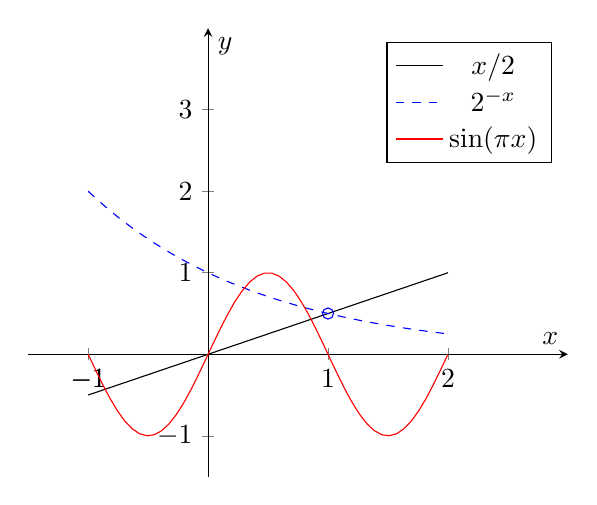
\begin{tikzpicture}
		\begin{axis}
			[
			legend pos= north east,
			axis lines = center,
			domain=-1:2,
			xlabel=$x$,
			xmin=-1.5,
			xmax=3,
			xtick={-1,-1,0,1,2},
			ylabel=$y$,
			ymin=-1.5,
			ymax=4,
			ytick={-1,0,1,2,3},
			samples=50,
			]
			\addplot [] {x/2};
			\addplot [blue,dashed] {2^(-x)};
			\addplot [red] {sin(deg(pi*x))};
			\addplot [blue, mark = o] coordinates {( 1, 1/2)};
			\legend{$x/2$,$2^{-x}$,$\sin(\pi x)$}
		\end{axis}
		\end{tikzpicture}
		\caption{Graphs of three analytical functions.}
		\label{fig:analytical}
	\end{figure}
	%
	
\end{document}
